\documentclass[conference]{IEEEtran}
\IEEEoverridecommandlockouts

% *** PACKAGES ***
\usepackage{cite}
\usepackage{amsmath,amssymb,amsfonts}
\usepackage{algorithmic}
\usepackage{graphicx}
\usepackage{textcomp}
\usepackage{xcolor}
\usepackage{siunitx}
\usepackage{float}
\usepackage{geometry}
\usepackage[spanish,english]{babel}  % Añade soporte para español
\usepackage[utf8]{inputenc}  % Soporte para caracteres especiales
\usepackage{fancyhdr}
\usepackage{graphicx}
\usepackage{indentfirst}
\usepackage{listings}
\usepackage{xcolor}
\usepackage{amsmath}
\usepackage{enumitem}
\usepackage{siunitx}
\usepackage{hyperref}
\graphicspath{{./}{imagenes ensayo de ingenieria/}{imagenes_circuitos/}{imagenes_placa/}{imagenes_potencia/}{imagenes_varias/}}


\begin{document}

\title{Desarrollo de \textit{ESC} para motores \textit{BLDC} sin sensores de posición, basado en microcontrolador de la gama \textit{STM32}}

\author{Francisco Castel\\\normalsize Facultad de Ingeniería - UNCUYO \\\normalsize Mendoza, Argentina\\\normalsize castel.francisco@uncuyo.edu.ar \\\normalsize\url{https://github.com/fcastel2002}}

\maketitle


\begin{abstract}
Este trabajo presenta el desarrollo e implementación de un Controlador Electrónico de Velocidad (ESC) \textit{sensorless} para motores \textit{BLDC/PMSM} utilizando microcontroladores STM32. El diseño se centra en un enfoque de bajo costo y complejidad reducida, basado en la detección de cruces por cero (ZCP) de la fuerza contraelectromotriz mediante comparadores analógicos, complementado con un control PI para la regulación de velocidad. La arquitectura propuesta aprovecha periféricos nativos del STM32F103C8T6 (\textit{timers} avanzados, ADC, \textit{UART} y memoria \textit{Flash}), lo que minimiza la carga computacional y aumenta la robustez del sistema. Se implementó una estrategia de arranque basada en modulación SPWM trifásica en lazo abierto, que asegura una transición estable hacia el régimen \textit{sensorless}. Asimismo, se desarrolló una máquina de estados modular que gestiona los distintos modos de operación (IDLE, RUNNING, CLOSED-LOOP, CONFIG, entre otros), mejorando la escalabilidad y confiabilidad del \textit{firmware}. Los ensayos experimentales con motores \textit{BLDC} extraídos de discos rígidos demostraron un rango de operación entre 100 y 5500 rpm, estabilidad térmica en la etapa de potencia basada en L298N, y un control adecuado bajo condiciones de carga predecible. El prototipo constituye una base funcional para aplicaciones donde la simplicidad y la eficiencia prevalecen sobre la necesidad de control dinámico avanzado, tales como ventiladores, sistemas de bombeo y pequeños vehículos eléctricos. Finalmente, se discuten limitaciones del enfoque reactivo y posibles mejoras mediante técnicas predictivas o híbridas, apuntando hacia futuras implementaciones con mayor robustez e integración industrial.
\end{abstract}

\title{\textbf{Microcontroladores y Electrónica de Potencia}

\vspace{0.5cm}
Trabajo Integrador:
\vspace{0.3cm}

\textit{Controlador Electrónico de Velocidad (ESC) para motores BLDC - PMSM sin sensores de posición}}
\author{Francisco Castel \\ \normalsize{Legajo: 13784}}{}
\date{Febrero 2025}

\maketitle

\section{Introducción}


Los motores \textit{BLDC-PMSM }(\textit{Brushless DC - Permanent Magnet Synchronous Motors}) representan una tecnología fundamental en aplicaciones que requieren alta eficiencia y control preciso, desde electrodomésticos hasta vehículos eléctricos y sistemas industriales. Su alta densidad de potencia, eficiencia superior (típicamente 85-95\%) y mayor vida útil los han convertido en la pieza fundamental durante el desarrollo y evolución de los drones, donde la relación potencia-peso es crítica. Es por esto que la motivación principal de este trabajo es la de entender profundamente el funcionamiento de este tipo de motores y las estrategias y técnicas de control del mismo.

Para lograr este objetivo se propuso la realización de un Controlador Electrónico de Velocidad (ESC) ya que prometía ser un desafió interesante y con cierta complejidad.

La evolución de las técnicas \textit{sensorless} ha sido notable desde que Iizuka et al. [1] propusieron en 1985 un método basado en la detección del \textit{Zero Crossing Point} (ZCP) mediante comparadores externos, estableciendo las bases para futuros desarrollos. Posteriormente, técnicas como las descritas por [2] mejoraron la precisión mediante la medición de \textit{BEMF} durante la ventana de \textit{PWM OFF}. Un avance significativo llegó con Chen [3], quien simplificó el \textit{hardware} necesario aprovechando el voltaje de línea, eliminando la necesidad de circuitos analógicos adicionales para el cálculo del instante de conmutación.

Actualmente, el Control de Campo Orientado (FOC) representa el estado del arte, ofreciendo control preciso de par y velocidad en un amplio rango operativo. Sin embargo, el FOC requiere algoritmos complejos que demandan mayor capacidad computacional y una medición de corriente con SNR superior a 40dB, lo que incrementa los costos de implementación.

El objetivo del presente trabajo es proporcionar un método sencillo y económico para el control \textit{sensorless} de motores BLDC/PMSM utilizando microcontroladores STM32. El enfoque se basa en la detección de cruces por cero mediante circuitos analógicos simples, complementados con un control PI para regular la velocidad. Esta implementación aprovecha los periféricos del STM32F103C8T6 (ADC, \textit{timer} avanzados, etc) para minimizar la carga computacional, resultando ideal para aplicaciones de ventilación y movimiento de aire donde no se requiere control de posición ni alto par de arranque. El método es aplicable en sistemas de baja y media potencia con velocidades mínimas de operación superiores al 15-20\% de la nominal.

Este documento está organizado en secciones que cubren: fundamentos teóricos del control \textit{sensorless}, diseño del hardware basado en STM32, implementación del algoritmo de detección y control, resultados experimentales, y conclusiones con recomendaciones para trabajos futuros.

\subsection{Principio de funcionamiento de motores BLDC - PMSM}
Cuando hablamos de motores sin escobillas, existen principalmente dos tipos, los motores con una \textit{BEMF} trapezoidal, categorizados como BLDC, y los que presentan una \textit{BEMF} sinusoidal, como \textit{PMSM}. Ambos difieren de los motores DC con escobillas en que la conmutación debe realizarse de forma electrónica, y no se realiza por la construcción del mismo. Esta diferencia en la forma de onda de la \textit{BEMF} se debe principalmente a la distribución del bobinado y la configuración del campo magnético del rotor: los \textit{BLDC} típicamente utilizan bobinados concentrados y magnetización radial, mientras que los PMSM emplean bobinados distribuidos y, en muchos casos, magnetización sinusoidal.

\begin{figure}[H]
    \centering
    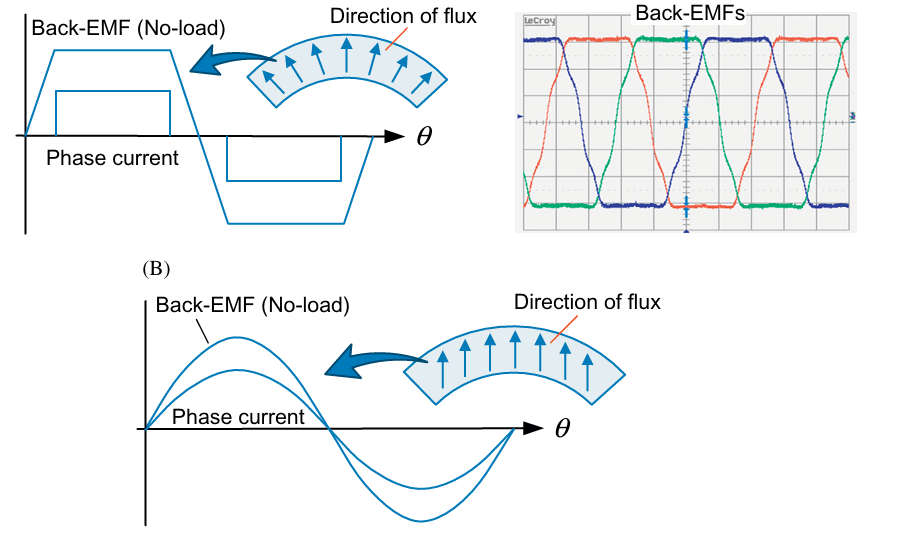
\includegraphics[width=1\linewidth]{imagenes_varias/bldc-pmsm.png}
    \caption{Diferencia sustancial entre BLDC y PMSM}
    \label{fig:bldc-pmsm-comparison}
\end{figure}
\subsubsection{Métodos de detección de cruces por cero}

La detección de los cruces por cero (ZCP) de la \textit{BEMF} constituye el método más implementado para el control \textit{sensorless} de motores BLDC. Este punto ocurre cuando la BEMF cambia de polaridad, lo que corresponde a una posición específica del rotor, generalmente desfasada 30° eléctricos del punto óptimo de conmutación.

\paragraph{Detección directa de \textit{BEMF}}
El método clásico propuesto por Iizuka et al. \cite{Iizuka1985} utiliza comparadores analógicos para detectar el instante en que la BEMF cruza el nivel de referencia (generalmente el punto neutro virtual). Esta técnica requiere circuitería de acondicionamiento para:

\begin{itemize}
    \item Filtrar el ruido de conmutación
    \item Crear un punto neutro virtual para comparación
    \item Generar una señal de interrupción al microcontrolador
\end{itemize}
Mas adelante en el presente trabajo, se expresa la elección de este método.
\paragraph{Método de integración de la tercera armónica}
Esta técnica, desarrollada por Moreira en el 96'\cite{Moreira1996}, aprovecha el hecho de que la suma de las tres \textit{BEMF} contiene una tercera armónica significativa. La integración de esta componente proporciona información de posición más robusta frente al ruido, aunque requiere un procesamiento adicional.

\paragraph{Método de terminal único}
Propuesto por Chen et al. \cite{Chen2007}, este enfoque simplifica la implementación hardware al utilizar solo un terminal para la medición de voltaje de línea. La principal ventaja es la reducción de componentes externos y la posibilidad de implementación completa en microcontroladores con suficientes recursos de ADC.

\paragraph{Detección mediante PWM sincronizado}
Este método, particularmente adecuado para implementaciones en microcontroladores, muestrea la BEMF durante los períodos de apagado del PWM, cuando la corriente de fase es mínima. La técnica requiere una sincronización precisa entre el PWM y la secuencia de muestreo del ADC, factible en microcontroladores avanzados como la familia STM32 que ofrecen disparo sincronizado entre periféricos \cite{STM32F103_RM}.

\section{Esquema tecnológico}
\begin{figure}[H]
    \centering
    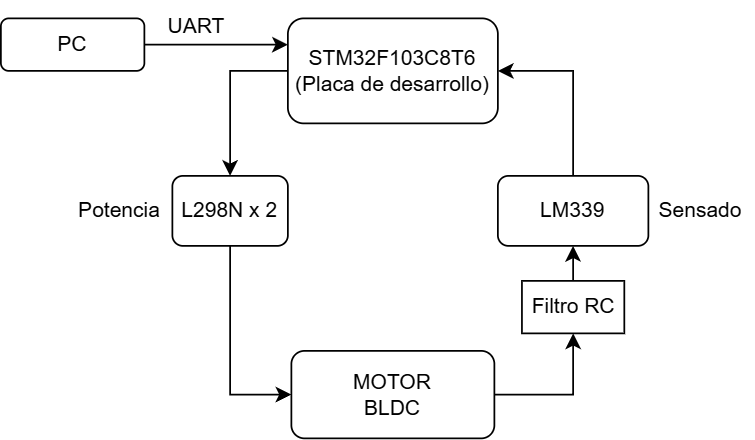
\includegraphics[width=0.85\linewidth, keepaspectratio]{imagenes_varias/esquema tecnologico.drawio.png}
    \label{fig:enter-label}
\end{figure}


\subsection{Detalle de módulos}

 
\subsubsection{Etapa de potencia: L298N}

La etapa de potencia se implementó utilizando dos módulos basados en el circuito integrado L298N \cite{STMicroelectronics_L298N}, configurados para proporcionar tres medios puentes H necesarios para la conmutación trifásica del motor BLDC. Cada medio puente se controla mediante dos señales: una para el transistor superior y otra para el inferior.
Este módulo presenta las siguientes características:
\begin{itemize}
    \item Voltaje de salida: 5V - 35V
    \item Voltaje lógico: 5V - 7V
    \item Corriente máxima por canal: 2A
    \item Potencia máxima de disipación: 25W
\end{itemize}

\begin{figure}[H]
    \centering
    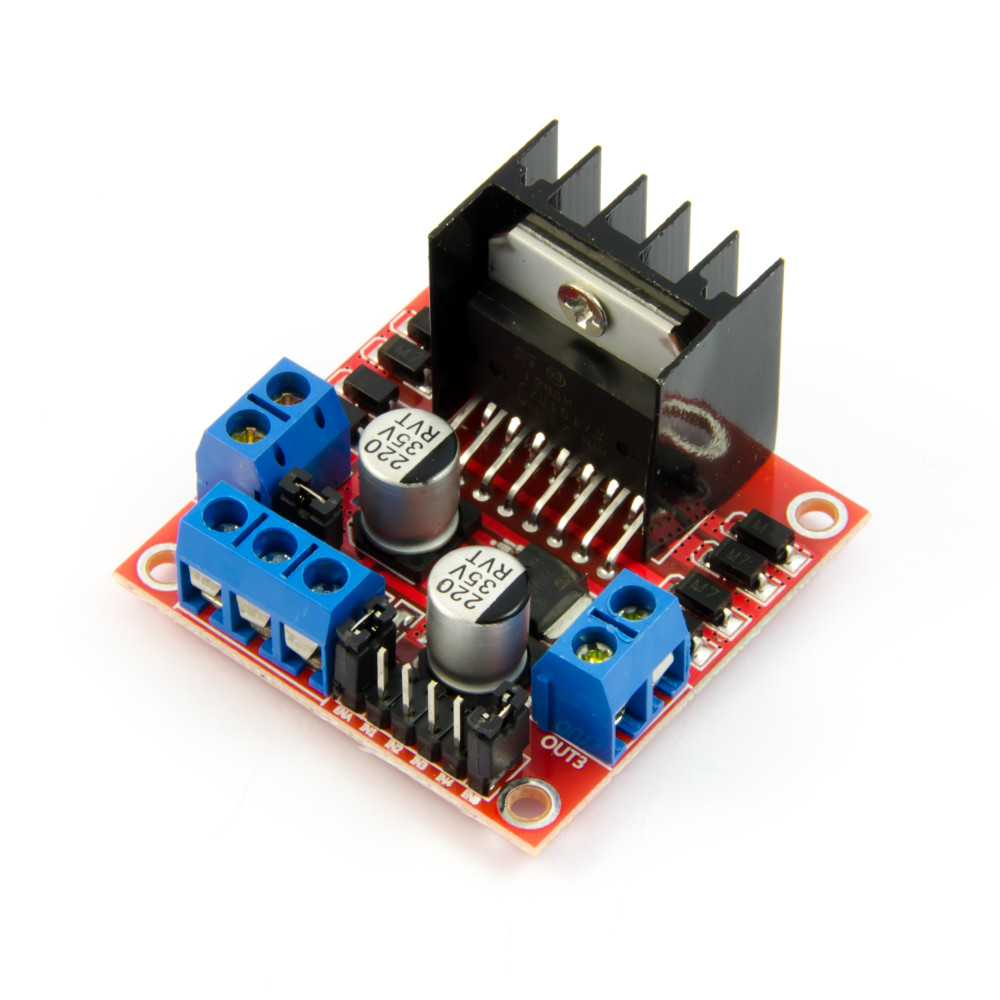
\includegraphics[width=0.5\linewidth]{imagenes_potencia/L298N.png}
    \caption{Módulo comercial basado en L298N y sus respectivas etapas de filtrado y feedback.}
    \label{fig:enter-label}
\end{figure}
\subsubsection{Motor utilizado}
Para las pruebas se utilizaron dos motores sin escobillas sacados de discos rígidos antiguos, estos fueron una gran elección debido a la alta disponibilidad como chatarra. No fue posible probar el sistema con motores BLDC de alto rendimiento como los presentes en drones comerciales. 
Así como estos motores son sencillos de conseguir, tambien es muy dificil de encontrar alguna referencia de ellos en internet ya que la mayoria de códigos de referencia y/o números, eran mas bien códigos internos y no existen como tales, por lo que no se consiguieron datos del motor como tal. Aunque un parámetro que si era relevante para saber si el algoritmo estaba funcionando de una forma adecuada era la velocidad máxima, y la de los discos rígidos antiguos solía ser de no más de 5400 rpm, a diferencia de los actuales que llegan a las 7200 rpm.

Para que se noción de la antigüedad de estos motores, los discos duros de los que fueron extraídos usaban motores paso a paso para mover la aguja de lectura.

\begin{figure}[H]
    \centering
    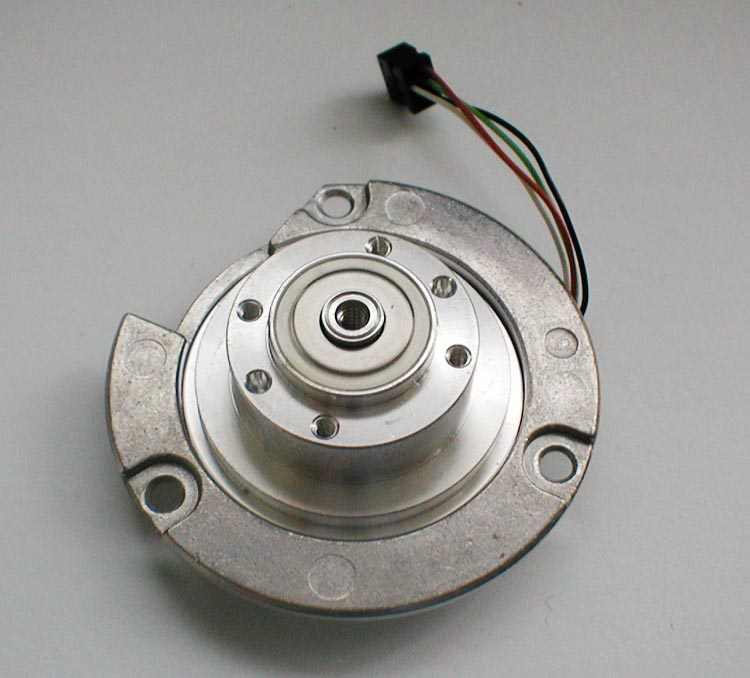
\includegraphics[width=0.5\linewidth]{imagenes_varias/motor_bldc.png}
    \caption{Motor extraido de un disco rígido antiguo}
    \label{fig:enter-label}
\end{figure}
\subsubsection{Circuito externo de detección}

Para la detección de cruces por cero de la fuerza contraelectromotriz (BEMF), se implementó el método propuesto por Iizuka \cite{Iizuka1985}, que utiliza comparadores analógicos para detectar los instantes en que la BEMF de la fase flotante cruza el nivel del punto neutro virtual. La \cref{fig:zero_crossing_2} muestra el circuito implementado.

En esta configuración, las resistencias R4-R6 (10 k$\Omega$) crean un punto neutro virtual, lo que flexibiliza el tipo de bobinado de motor, ya que sea Estrella o Delta (acceso al neutro real o no) se utilizan solo las terminales de las tres fases. Luego las resistencias R1-R3 (10k$\Omega$) y capacitores C1, C2 y C3 (47 nF)  forman una etapa de filtrado para reducir el ruido de conmutación y propio del motor. Los comparadores del LM339 \cite{TI_LM339} detectan el momento exacto del cruce por cero (aun así se dota de histéresis  mediante resistencias de 100 k$\Omega$), generando flancos que son capturados por los canales de Input Capture (IC\_CH1, IC\_CH2 e IC\_CH3) del temporizador del microcontrolador.

Se seleccionó el LM339 debido a su salida de colector abierto, que permite una interfaz segura entre los 12V del circuito de potencia y los 3.3V del STM32F103C8T6, sin necesidad de circuitos adicionales de adaptación de nivel.
\begin{figure}[H]
    \centering
    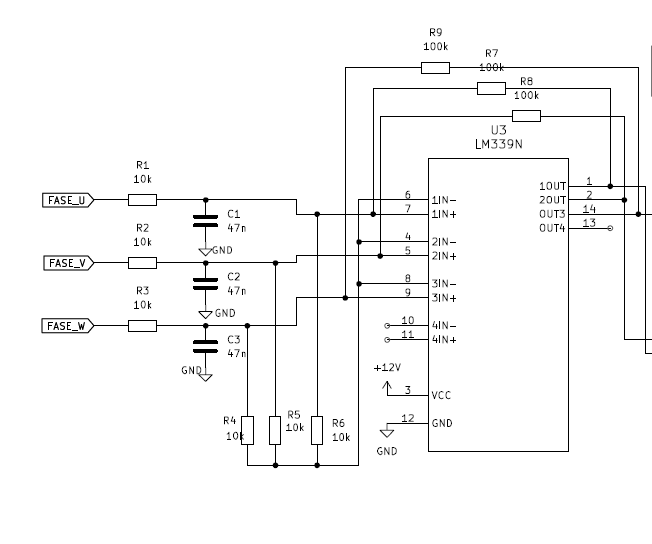
\includegraphics[width=1\linewidth]{imagenes_circuitos/esquematico_3_zc.png}
    \caption{Circuito implementado}
    \label{fig:zero_crossing_2}
\end{figure}
 Se decide la utilización de un comparador de collector abierto como el LM339 \cite{TI_LM339}  debido a su versatilidad al momento de interactuar con dispositivos de voltajes sumamente distintos al de alimentación, como en este caso, 12V contra los 3.3 V del STM32F103C8T6.


\section{Funcionamiento general}
El objetivo principal del controlador es el de lograr la consigna de velocidad en el motor, para ello debe recibir los cruces por cero y a partir de ellos realizar las conmutaciones correspondientes. El funcionamiento del firmware en sí es sencillo, lo que hace es:

\begin{enumerate}
    \item Rutina de arranque. 
    \item Realizar la conmutación cuando se recibe el flanco correspondiente desde el circuito comparador.
    \item Medir el periodo entre dos flancos de subidas de una misma fase.
    \item Cada cierto tiempo (regido por la velocidad máxima) actualizar la salida PWM mediante un control PI.
\end{enumerate}

\begin{figure}[H]
    \centering
    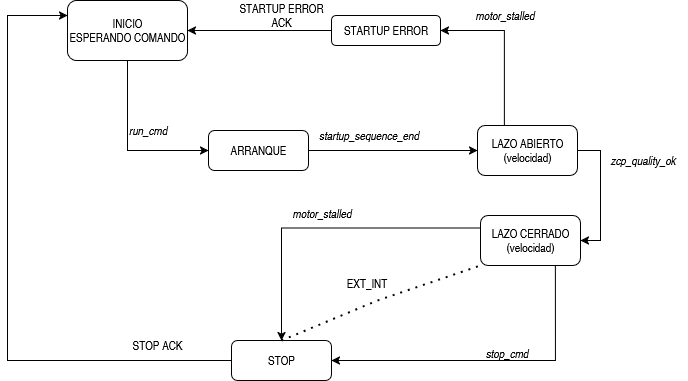
\includegraphics[width=1\linewidth]{imagenes_varias/df_light_revisado.drawio.png}
    \label{fig:diagrama-flujo}
\end{figure}
Pero esto no es suficiente para una conmutación robusta, fue sumamente necesario incluir un algoritmo sencillo de detección de la consistencia de la señal del cruce por cero. Esto es crucial para sobre todo el funcionamiento en lazo cerrado.
\section{Programación}
\subsection{Configuración de periféricos del microcontrolador}

El microcontrolador STM32F103C8T6 se configuró para realizar tanto la detección de cruces por cero como la generación de señales de control para los puentes H:

\begin{itemize}
    \item \textbf{\textit{timer} 2:} Configurado con tres canales en modo Input Capture para detectar los flancos provenientes de los comparadores. Este enfoque, en lugar de utilizar interrupciones externas (EXTI), permite medir directamente el período entre cruces por cero, facilitando el cálculo de la velocidad del motor y la temporización precisa de la conmutación.
    
    \item \textbf{\textit{timer} 1:} Utilizado como generador PWM para controlar los transistores superiores de los medios puentes. Se configuró para operar en un rango de frecuencias entre 10 y 24 kHz (no fue necesaria la implementación de tiempo muerto dado que el retraso propio de la conmutación proporciona una especie de dead time).
    
    \item \textbf{UART1:} Periférico UART configurado a 115200 de baudrate utilizado en modo interrupción.
    
\item \textbf{CRC:} Periférico utilizado para la verificación de integridad de datos. Este módulo permite realizar cálculos rápidos de verificación, contribuyendo a la robustez en la transmisión y almacenamiento de parámetros críticos, se utiliza para la persistencia de parámetros en FLASH.

\item \textbf{Memoria Flash:} Utilizada para almacenamiento no volátil de parámetros de configuración y calibración del ESC. La memoria Flash permite conservar configuraciones esenciales entre reinicios o ciclos de alimentación. Permite al operario configurar su ESC como desee.
    
    
\end{itemize}
\subsubsection{Señales PWM}
La técnica PWM seleccionada corresponde a "PWM technique 1" en la \cref{fig:pwm-tech}, también conocida como PWM unipolar. En esta configuración, durante cada sector de 60° eléctricos, una fase se conecta al positivo mediante PWM, otra fase se conecta al negativo de forma permanente, y la tercera fase permanece flotante (desconectada).  
Se eligió esta técnica ya que la implementación de las demás técnicas, según Lai et al en \cite{Lai2011}, pueden cobrar sentido si se utiliza un método de sensado directo de la BEMF mediante ADC.

 \begin{figure}[H]
     \centering
     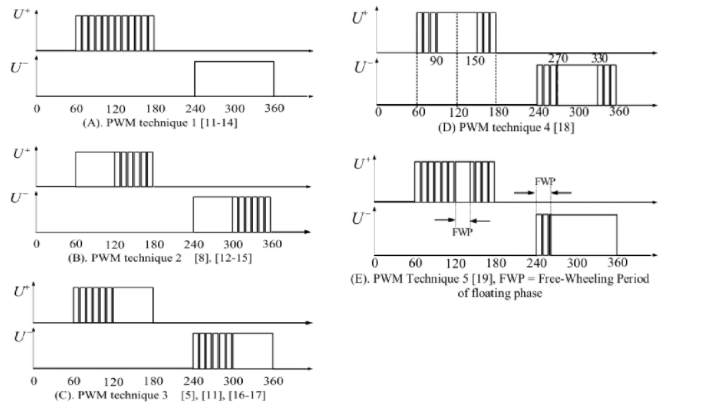
\includegraphics[width=0.95\linewidth]{imagenes_potencia/PWM_TECH2.png}
     \caption{Resumen de técnicas PWM para motores BLDCM.\cite{Lai2011}}
     \label{fig:pwm-tech}
 \end{figure}



\subsection{Estrategia de arranque}

El arranque representa uno de los mayores desafíos en el control \textit{sensorless} de motores BLDC, ya que a velocidad cero o muy baja no se genera suficiente BEMF para detectar la posición del rotor. En este trabajo se evaluaron diferentes estrategias de arranque antes de seleccionar la implementación final.

\subsubsection{Alternativas consideradas}

La técnica \textit{Align \& Go}, ampliamente documentada en la literatura, fue inicialmente considerada debido a su simplicidad de implementación. Sin embargo, esta técnica presenta una desventaja significativa: la posibilidad de que el rotor inicie su movimiento en dirección opuesta a la deseada. Si bien existen algoritmos para detectar y corregir esta situación, su implementación requiere una detección casi instantánea del sentido de rotación y una rápida inversión de la secuencia de conmutación, aumentando considerablemente la complejidad del sistema.

Otra alternativa analizada fue el método IPD (\textit{Initial Position Detection}), implementado por Meghana \textit{et al} en \cite{Meghana2020}, que permite un arranque desde velocidad cero mediante la detección de la posición inicial del rotor. A pesar de ser el método más utilizado en aplicaciones comerciales de control \textit{sensorless}, la complejidad de sus algoritmos y los requisitos de sincronización precisa entre periféricos lo situaron fuera del alcance de este trabajo.

\subsubsection{Solución implementada: SPWM en la etapa de arranque}

La estrategia de arranque adoptada se basa en un generador senoidal de tres fases mediante modulación por ancho de pulso senoidal (SPWM), implementado completamente en lazo abierto. Esta técnica consiste en:

\begin{enumerate}
    \item Precálculo de tres tablas senoidales desfasadas 120° eléctricos entre sí (una por fase), ajustadas al formato \texttt{Q15} y escaladas para facilitar su modulación en tiempo real.
    \item Generación periódica de valores PWM actualizados a partir de dichas tablas, mediante un temporizador auxiliar que actualiza el índice de fase a intervalos controlados.
    \item Aplicación de estas señales al puente inversor trifásico del motor, con habilitación de las tres fases y control de flotación durante toda la etapa de arranque.
    \item Incremento controlado de la frecuencia efectiva del campo rotante a través de la reducción progresiva del \texttt{ARR} (Auto-Reload Register) del temporizador auxiliar.
    \item Aumento gradual del valor de modulación (\texttt{mod\_q15}), que controla la amplitud de la señal aplicada, desde un valor inicial bajo ($\approx 20\%$) hasta una amplitud estable cercana al 100\%.
    \item Finalización automática del arranque tras un número fijo de iteraciones (\texttt{STARTUP\_ITERATIONS}), momento en el cual se realiza la transición controlada al modo de conmutación trapezoidal \textit{sensorless}.
\end{enumerate}

La lógica de control se implementa utilizando el temporizador TIM4 del STM32F103C8T6 para las actualizaciones periódicas de PWM, mientras que el generador de PWM (TIM1) continua modulando la señal SPWM. Durante el arranque, el sistema no requiere retroalimentación alguna del motor: no se evalúa la \textit{BEMF}, ni se mide corriente, ni se utiliza información de posición.

La transición al modo de operación \textit{sensorless} se realiza de forma determinista, tras agotar el tiempo definido para el arranque. En ese instante, se detiene la modulación SPWM, se deshabilitan momentáneamente las salidas, y se reinicializa el sistema para comenzar con la conmutación trapezoidal convencional, habilitando el sistema de detección de cruces por cero.

\subsubsection{Ventajas y limitaciones}

Esta aproximación presenta varias ventajas relevantes para la aplicación:

\begin{itemize}
    \item Permite un arranque suave y robusto, incluso en ausencia total de información de posición o velocidad.
    \item Es insensible a la posición inicial del rotor, gracias a la naturaleza continua del campo magnético rotante generado.
    \item Su implementación es simple y determinista: no requiere ajustes dinámicos durante el arranque, ni evaluación de condiciones de éxito o fallo.
\end{itemize}

Como limitación principal, el sistema no es capaz de detectar si el motor ha sincronizado efectivamente durante la etapa de arranque. El método asume que, al finalizar el tiempo definido, el rotor habrá sido capaz de seguir el campo magnético generado. Esto representa un riesgo en condiciones de carga elevada o con el rotor bloqueado, ya que la transición podría realizarse sin que el motor haya adquirido velocidad efectiva.

Cabe destacar, sin embargo, que si bien durante el arranque no se evalúa la consistencia de los cruces por cero debido a que la señal de \textit{BEMF} queda enmascarada por la modulación senoidal (haciendo que cualquier cruce detectado en esta etapa sea irrelevante o espurio), el sistema implementa una verificación posterior. Tras completarse el tiempo de arranque y al entrar al modo \textit{sensorless}, si los cruces por cero detectados no presentan la coherencia esperada, se considera fallida la sincronización y se vuelve automáticamente a ejecutar la maniobra de arranque desde cero. Esta estrategia añade una capa de robustez frente a condiciones anómalas sin complejizar la lógica de control durante el arranque propiamente dicho.

\subsection{Conmutación}
Para conmutación de las fases, se optan dos estrategias cruciales para no perder la sincronización tan buscada desde la etapa de arranque entre los cruces por cero, la posición del rotor y los pasos de la conmutación.

\subsubsection{Fase flotante como variable global}
Un problema que surgía al momento de utilizar el método de Iizuka es que si no se asignaba un orden de prioridad a las interrupciones era factible que uno de los canales detectara una segunda interrupción antes de que el canal de la fase que nos interesa (la fase flotante) detectase su flanco, provocando esto una conmutación a destiempo. Por esto se deciden crear tres variables booleanas (float\_U; float\_V y float\_W) que se encargan de informar al callbak de interrupciones de cual será la próxima fase flotante, es decir, el próximo canal que debe atender.
Por ejemplo, para el paso de conmutación que energiza las fases U y V (+U -V) el trio de variables tomaría los siguientes valores:
\begin{itemize}
    \item float\_U = false
    \item float\_V = false
    \item float\_W = true
\end{itemize}
Agregando así un condicional adicional al callback de interrupción.
\subsubsection{Alternado de polaridad del input capture}
Un factor indispensable a tener en cuenta durante el desarrollo de la conmutación fue el de la necesidad de que los canales del input capture correspondientes a cada fase pudiesen captar tanto flancos de bajada como de subida, lamentablemente esto no esta permitido para el canal 3 del \textit{timer} 1 (aun siendo este un \textit{timer avanzado}) por lo que este inconveniente se soluciono cambiando la polaridad de cada canal de forma alternada, es decir que, por ejemplo, el canal que corresponde a la fase U, para la primer posicion dentro de la secuencia se establece con polaridad de flanco de bajada, y luego para el proximo paso donde la fase U es flotante, se establece la polaridad de flanco de subida, esto se repetirá para cada canal. Esta implementación no solo solucionó las incapacidades del \textit{timer} 1, si no que propuso más robustez al sistema previniendolo de falsos cruces por cero dados por posible ruido, así, es imposible que un flanco de bajada sea detectado previo a otro flanco de bajada del mismo canal.
\setlength{\tabcolsep}{3pt} % valor más pequeño que el default (6pt)
\begin{table}[htbp]
  \centering
  \caption{Secuencia de conmutación de 6 pasos para motor BLDC}
  \label{tab:bldc_commutation}
  \resizebox{\columnwidth}{!}{%
    \begin{tabular}{|c|ccc|ccc|c|ccc|}
      \hline
      \multirow{2}{*}{\textbf{Paso}} & \multicolumn{3}{c|}{\textbf{Enable}} & \multicolumn{3}{c|}{\textbf{PWM}} & \multirow{2}{*}{\textbf{Polaridad}} & \multicolumn{3}{c|}{\textbf{Flotantes}} \\
      \cline{2-7}\cline{9-11}
      & \textbf{U} & \textbf{V} & \textbf{W} & \textbf{U} & \textbf{V} & \textbf{W} & & \textbf{U} & \textbf{V} & \textbf{W} \\
      \hline
      POS\_UV & 1 & 1 & 0 & PWM & 0 & - & Fall(CH1) & No & No & Sí \\
      POS\_UW & 1 & 0 & 1 & PWM & - & 0 & Rise(CH3) & No & Sí & No \\
      POS\_VW & 0 & 1 & 1 & - & PWM & 0 & Fall(CH2) & Sí & No & No \\
      POS\_VU & 1 & 1 & 0 & 0 & PWM & - & Rise(CH1) & No & No & Sí \\
      POS\_WU & 1 & 0 & 1 & 0 & - & PWM & Fall(CH3) & No & Sí & No \\
      POS\_WV & 0 & 1 & 1 & - & 0 & PWM & Rise(CH2) & Sí & No & No \\
      \hline
    \end{tabular}%
  }
\end{table}
\subsection{Sistema de máquina de estados}

La máquina de estados constituye la columna vertebral del controlador, gestionando las transiciones entre los diferentes modos de operación.

La función \texttt{handleState()} implementa un patrón de diseño basado en estados que permite:

\begin{itemize}
    \item Separar claramente la lógica para cada modo de operación
    \item Gestionar transiciones controladas entre estados
    \item Mantener activas solo las interrupciones necesarias en cada estado
\end{itemize}
\section{Resumen del funcionamiento de la máquina de estados}

El módulo de la máquina de estados (`state\_machine.c`) implementa el control centralizado del ESC mediante una estructura clara y robusta basada en estados. Las funciones y características principales son:

\begin{itemize}

\item \textbf{handleState():} Gestiona la transición entre estados, procesando eventos internos y externos, asegurando una ejecución ordenada y segura del ESC.

\item \textbf{Estados clave:}
\begin{itemize}
  \item \textbf{IDLE:} Estado inicial o de espera sin actividad del motor.
  \item \textbf{PROCESS\_COMMAND:} Procesa comandos recibidos desde el módulo de comunicación.
  \item \textbf{FOC\_STARTUP:} Maneja la secuencia inicial de arranque.
  \item \textbf{RUNNING:} Estado operativo básico, gestionando velocidad abierta.
  \item \textbf{CLOSEDLOOP:} Control operativo avanzado con ajuste automático por realimentación.
  \item \textbf{CONFIG:} Realiza configuraciones recibidas por comandos externos.
  \item \textbf{READY:} Preparación intermedia para el control de lazo cerrado.
  \item \textbf{STOPPED:} Estado de detención del motor.
  \item \textbf{FINISH:} Finaliza operaciones y retorna a IDLE.
  \item \textbf{HARD\_ERROR:} Manejo de errores críticos que requieren intervención.
\end{itemize}

\end{itemize}

La máquina de estados garantiza un control robusto, previniendo errores críticos mediante transiciones claras y supervisadas, y actúa como núcleo central que coordina la interacción y comunicación efectiva entre todos los módulos del sistema. Su estructura es fácilmente escalable, facilitando la incorporación de nuevos estados y eventos según sea necesario.

\subsection{Funciones mas importantes del control}
\begin{itemize}

\item \textbf{\textit{commutation}()} \par
Controla la secuencia de activación/desactivación de las fases U, V, y W del motor brushless según el paso actual de conmutación.

Establece las polaridades adecuadas y asigna valores PWM específicos a cada fase según la posición del rotor.

\item \textbf{\textit{zero\text{\_}crossing}()} \par
Gestiona el control del motor mediante la detección de cruces por cero (\textit{Zero Crossing Points - ZCP}).

Realiza la conmutación del motor en cada cruce por cero detectado en cualquiera de las fases.

Actualiza la velocidad usando mediciones tri-fase para calcular un promedio por consenso entre las fases (método robusto).

\item \textbf{\textit{pi\_control}()} \par
Implementa un controlador Proporcional-Integral (PI) para ajustar el PWM del motor según un setpoint de velocidad.

Utiliza parámetros configurables (KP, KI) para el control fino de la velocidad y limita la salida PWM dentro de rangos seguros.


\item \textbf{\textit{check\_motor\_status}()} \par
Monitorea periódicamente el estado operativo del motor.

Detecta condiciones de bloqueo (stall) mediante la comprobación de tiempo desde el último cruce por cero válido.
Establece una bandera (motor\_stalled) para indicar situaciones críticas.

\item \textbf{\textit{stop\_motor}()} \par
Maneja el procedimiento para detener el motor en dos modos:

Detención gradual (modo normal).

Detención inmediata de emergencia (modo crítico), con cambio de dirección temporal para frenado rápido.


\item \textbf{\textit{calculate\_consensus\_speed}()} \par
Calcula la velocidad promedio por consenso utilizando mediciones consistentes de múltiples fases, lo que mejora significativamente la robustez ante ruidos o fallos ocasionales en la detección de cruces por cero.


\end{itemize}

\subsection{Sistema de comunicación}

El controlador implementa un protocolo de comunicación basado en comandos textuales a través de UART, permitiendo la configuración y monitorización del sistema.

\subsubsection{Resumen del funcionamiento de la comunicación}

El módulo de comunicación (`comm.c`) implementa la interfaz UART para interacción externa con el ESC. Las funciones más importantes son:

\begin{itemize}

\item \textbf{\textit{commInit}():} Inicializa el buffer de recepción y comienza la recepción por interrupción usando UART.

\item \textbf{\textit{processUartData}():} Lee y procesa bytes recibidos del buffer circular. Detecta comandos completos al recibir caracteres finales como \texttt{\textbackslash r} o \texttt{\textbackslash n}, almacenándolos para su ejecución.

\item \textbf{\textit{processCommand}():} Analiza comandos recibidos, los valida sintácticamente y determina la acción a realizar, pudiendo ejecutar acciones como RUN, STOP, EMERGENCY\_STOP o ajustes específicos como la frecuencia PWM.

\item \textbf{\textit{executeCommand}():} Ejecuta la acción indicada en el comando analizado (por ejemplo, configurar la frecuencia PWM o iniciar la maniobra de arranque FOC), devolviendo un estado de confirmación.

\item \textbf{transmitirUART():} Envía respuestas por UART usando transmisiones no bloqueantes por interrupción, informando estados o errores al usuario externo.


\end{itemize}

Este módulo asegura una comunicación robusta y eficiente con la interfaz externa, permitiendo el control dinámico del ESC mediante comandos estructurados. Además, su diseño es altamente escalable, ya que permite fácilmente la incorporación de nuevas acciones y parámetros para extender o adaptar el conjunto de comandos disponibles.


\section{Etapas de montaje y ensayos realizados}

En esta sección se describen las principales etapas del montaje del sistema ESC y los ensayos efectuados para verificar su funcionamiento.
\begin{figure}[H]
\centering
    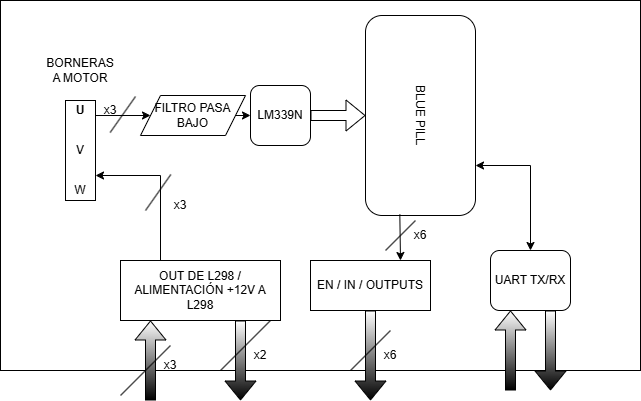
\includegraphics[width=0.5\textwidth]{imagenes_placa/diagrama_conceptual.png}
    \caption{Esquemático conceptual de conexiones y partes del prototipo}
    \label{fig:diagrama_conceptual}
\end{figure}

\begin{figure}[H]
    \centering
    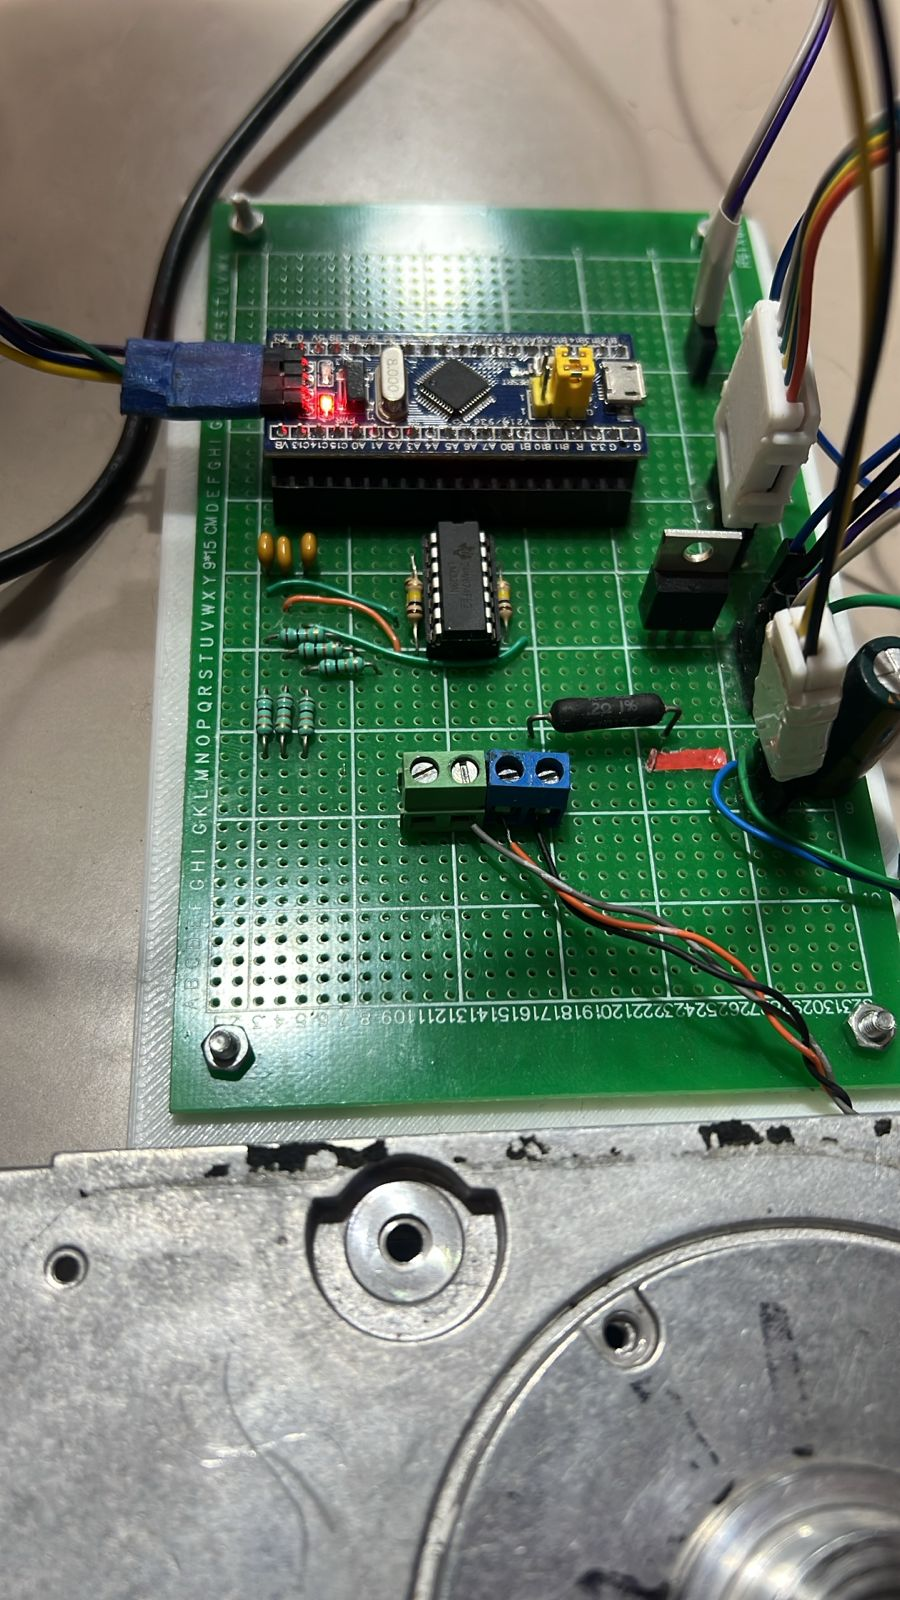
\includegraphics[width=0.4\textwidth]{imagenes_placa/placaprincipal_1.jpg}
    \caption{Montaje del circuito lógico en la placa de prototipado.}
    \label{fig:montaje_placa}
\end{figure}

\begin{figure}[H]
    \centering
    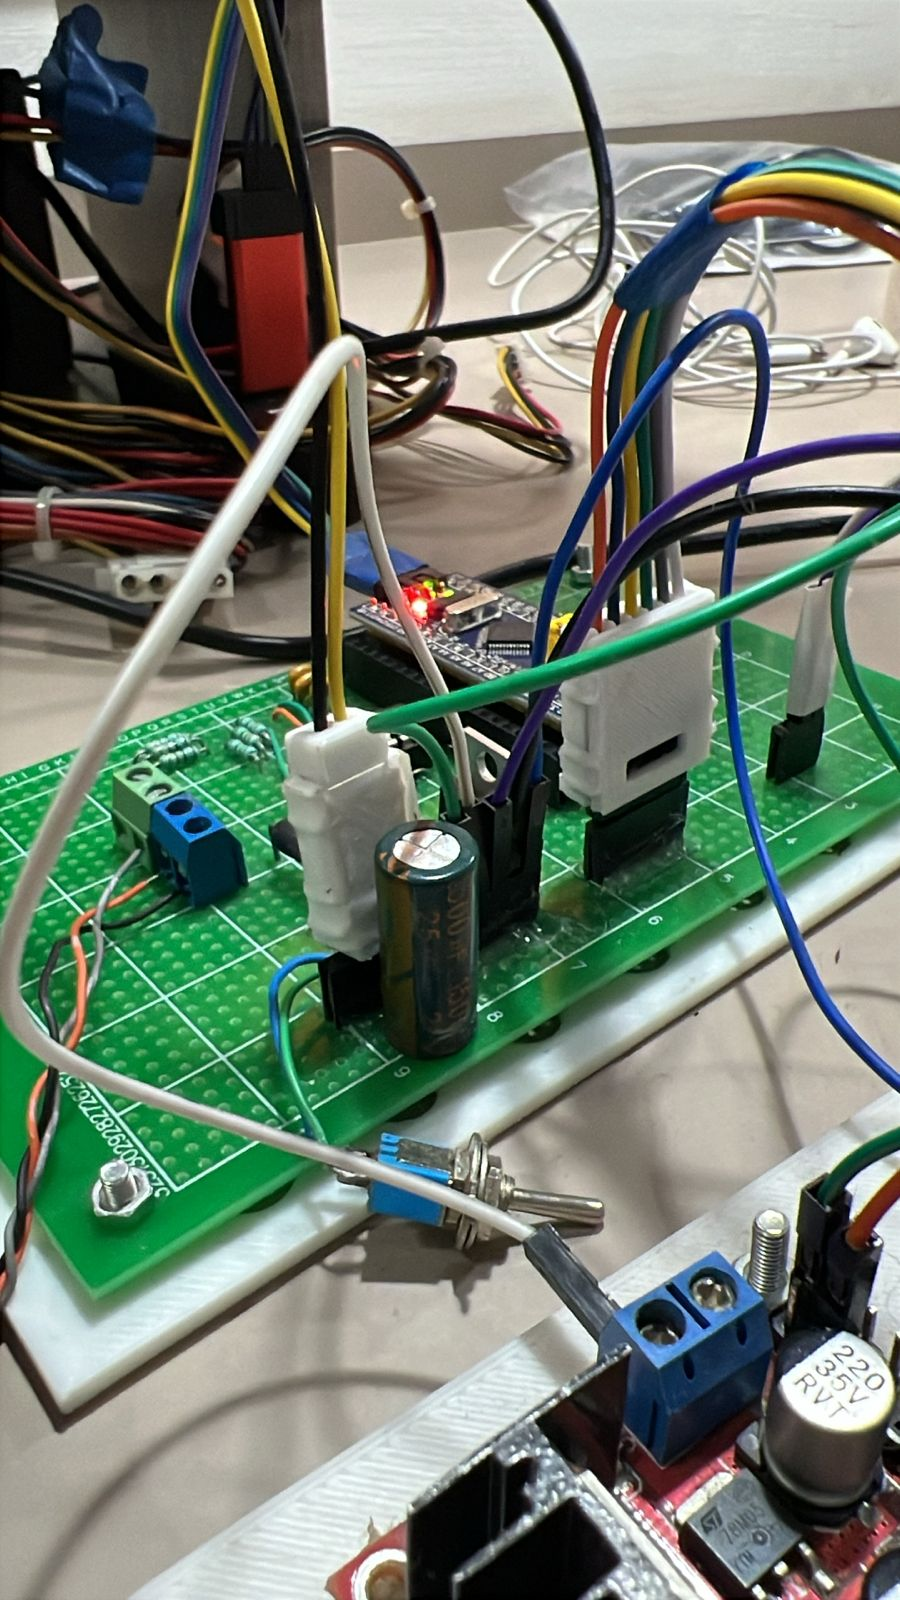
\includegraphics[width=0.5\textwidth]{imagenes_placa/placaprincipal_2.jpg}
    \caption{Otra vista del circuito lógico.}
    \label{fig:placa_2}
\end{figure}
En la imagen \ref{fig:placa_2} y \ref{fig:montaje_placa} se puede ver la protección a polaridad inversa mediante un Diodo Schottky y un capacitor de gran capacidad (1500 uF) para protección contra picos de corriente y estabilidad del MCU.

\begin{figure}[H]
    \centering
    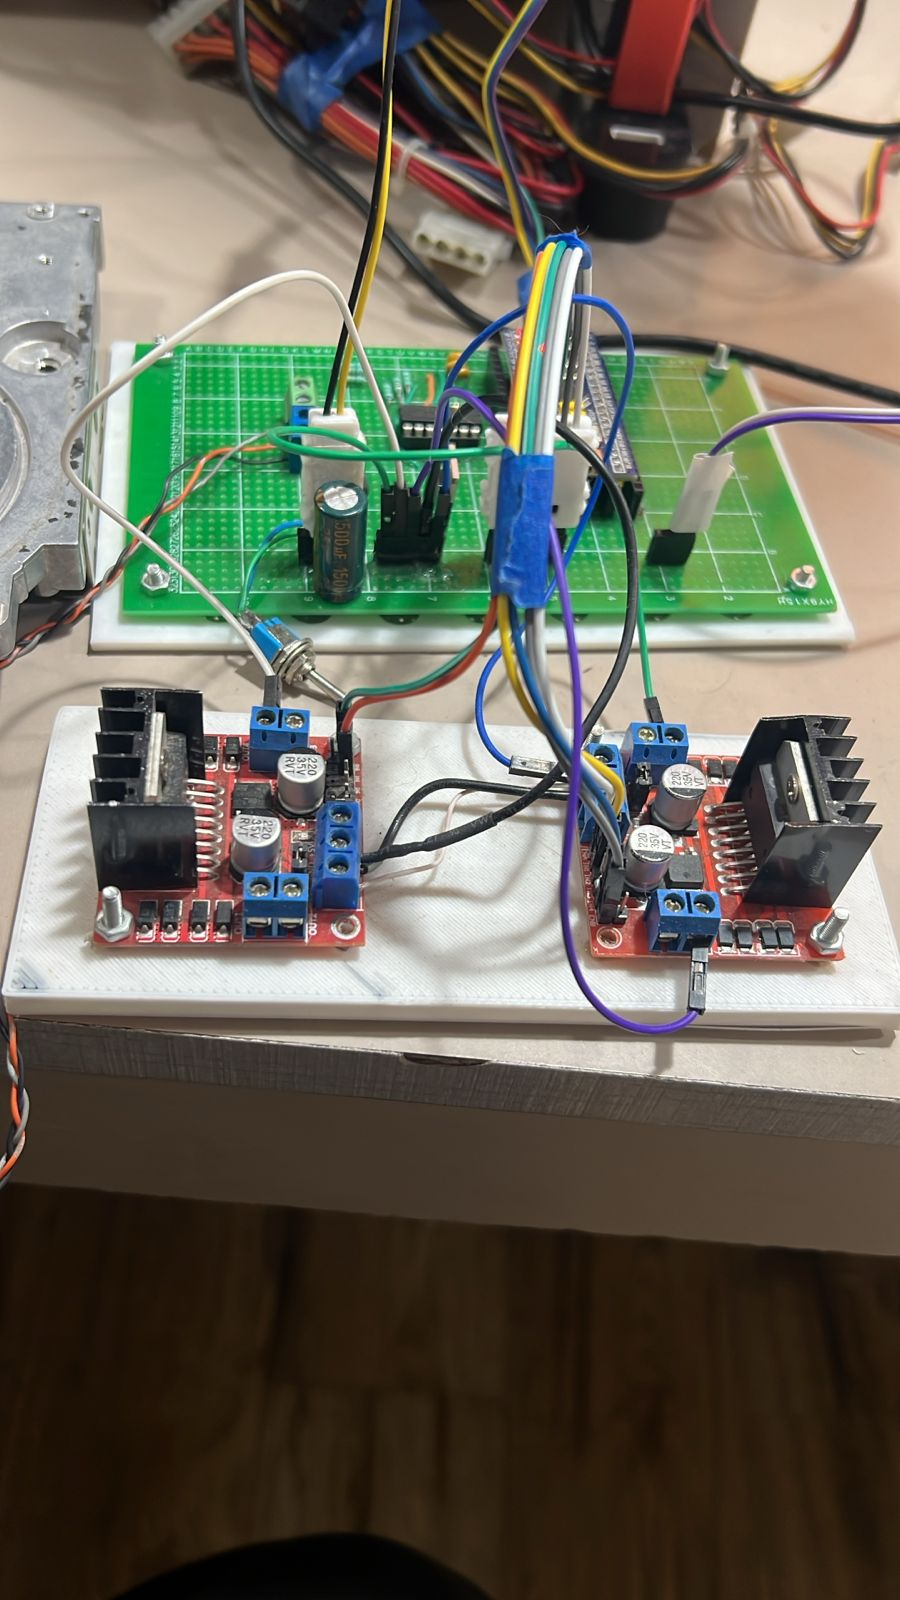
\includegraphics[width=0.5\textwidth]{imagenes_placa/todo_1.jpg}
    \caption{Etapa de potencia (2x L298N) y circuito lógico.}
    \label{fig:placa_potencia}
\end{figure}
Debe entenderse que un prototipo final no tendría la etapa de potencia separada en módulos como este caso, sino mas bien en una misma placa, la etapa de potencia y la etapa de control.

\section{Resultados y especificaciones finales}

Se presentan resultados cualitativos y cuantificativos del proyecto, obtenidos a partir de distintas pruebas.

\begin{itemize}
    \item Rango de operación: Sin ninguna carga, el motor, el cual nominalmente está diseñado en 5400 rpm, según las lecturas del osciloscopio muestra una velocidad máxima de 5500 rpm, y una velocidad mínima de 100 rpm.
    \item La etapa de potencia no presenta disipación térmica notable, con los disipadores presentes en los módulos L298, en términos generales, por lo mencionado, la temperatura de los mosfets no supera los 40°C.
    \item Limitante principal y próximo paso a mejorar: El hecho de que el sistema sea reactivo, y no predictivo, produce un comportamiento esperable, que no se puede confiar ciegamente en las lecturas de cruces por cero, por lo que es muy sensible a una desincronización. Se mejoraría este aspecto logrando un método predictivo, pero se soluciona por completo el enmascaramiento de la señal del cruce por cero tomando un enfoque de lectura de corrientes, sin entrar en algoritmo FOC.
    \item Control pobre en términos generales: No es posible realizar cambios bruscos de velocidad, ya que estos generan picos de corriente en la señal que distorsionan por completo la lectura de los cruces por cero, y debido a la naturaleza reactiva de estos, el control pierde sentido. Una solución muy interesante e investigada podría ser la implementación de control difuso para estas consignas de velocidad bruscas.
\end{itemize}

\section{Conclusiones. Ensayo de ingeniería de producto}

\subsection*{Aplicabilidad del sistema}

Si bien el ESC no está diseñado para aplicaciones que requieran precisión dinámica elevada o control activo de par, resulta especialmente adecuado para sistemas donde el control de velocidad sea el requerimiento principal y las condiciones de carga se mantengan dentro de márgenes predecibles.

Entre las aplicaciones posibles se incluyen:

\begin{itemize}
    \item Sistemas de bombeo de agua o fluidos industriales.
    \item Ventiladores centrífugos o axiales de media y baja potencia.
    \item Propulsión de pequeños drones o vehículos autónomos.
    \item Sistemas de refrigeración, circulación y climatización.
\end{itemize}

\subsection*{Análisis detallado: bomba centrífuga de agua}

Para validar más rigurosamente la viabilidad del controlador en una aplicación real, se analiza su desempeño esperado en el contexto del accionamiento de una bomba centrífuga.

Este tipo de carga presenta un perfil de par creciente con la velocidad, típicamente proporcional al cuadrado de la misma (\( T \propto \omega^2 \)). Además, las variaciones de carga durante el funcionamiento son suaves, lo que reduce las exigencias dinámicas del sistema de control. Asimismo, no se requiere inversión del sentido de giro ni regulación precisa del par instantáneo.

El ESC desarrollado cumple con los requerimientos básicos de esta aplicación:

\begin{itemize}
    \item \textbf{Arranque suave:} la rampa de frecuencia en modo SPWM permite una aceleración gradual, limitando los picos de corriente sin necesidad de sensado.
    \item \textbf{Control de velocidad estable:} tras el arranque, el sistema opera en lazo abierto con conmutación sincronizada a los cruces por cero, ofreciendo estabilidad suficiente en aplicaciones con dinámica lenta, como una bomba hidráulica.
    \item \textbf{Protección frente a bloqueo:} el firmware implementa un mecanismo de detección de pérdida de sincronía mediante el monitoreo de cruces por cero. Ante inconsistencias sostenidas, el sistema reinicia la secuencia de arranque o detiene la conmutación, funcionando como una protección frente a bloqueo mecánico.
    \item \textbf{Compatibilidad con el entorno operativo:} la topología sin sensores y el bajo número de componentes electrónicos favorecen la integración del controlador en entornos húmedos o de difícil acceso, donde la robustez y el bajo mantenimiento son prioridades.

\end{itemize}


\subsection*{Selección final de componentes y esquema de protección}

\begin{enumerate}[label=\textbf{\arabic*.}]
%---------------------------------------------------------------
\item \textbf{Motor de aplicación}
  \begin{itemize}
    \item Tipo: Brushless trifásico \textit{sensorless}, 12--24\,V.
    \item Ejemplo comercial: \emph{Turnigy D2830/11 1000\,KV} (100\,W continuo @ 12--14.8\,V, $I_\text{max} \approx 10$\,A).
  \end{itemize}

%---------------------------------------------------------------
\item \textbf{Etapa de potencia}
  \begin{itemize}
    \item \textbf{MOSFETs}: 6$\times$ \emph{IRLZ44N} (55\,V, \SI{47}{A}, $R_\text{DS(on)} \leq \SI{22}{\milli\ohm}$).  
    Montados sobre disipador común de aluminio (R\textsubscript{$\theta$SA}\,$\leq$\,2\,°C/W).  
    \item \textbf{Driver}: 3$\times$ \emph{IR2101S} (medio-puente alto/bajo, con bootstrap).  
    $V_\text{HB} \leq 600$\,V – sobredimensionado para 24\,V.  
    Capacidad de corriente de puerta: $\pm$2\,A (tiempo típico de carga $\approx$ 150\,ns para $Q_g \approx 100$\,nC).
    \item Resistores de puerta: $R_g = 10$--$12\,\Omega$ para amortiguación de \emph{ringing}.
  \end{itemize}

%---------------------------------------------------------------
\item \textbf{Controlador principal}
  \begin{itemize}
    \item \emph{STM32F103C8T6} (Cortex-M3, 72\,MHz), validado en el prototipo.
    \item Oscilador externo de 8\,MHz tipo \texttt{HC-49S} para mayor precisión temporal (PWM y captura).
  \end{itemize}

%---------------------------------------------------------------
\item \textbf{Fuente y filtro de entrada (24\,V\,DC)}
  \begin{itemize}
    \item Fuente conmutada industrial 24\,V / 6\,A (\emph{Mean Well LRS-150-24} o equivalente).
  \end{itemize}

%---------------------------------------------------------------
\item \textbf{Protección y aislamiento de señales}
  \begin{itemize}
    \item Para proteger el microcontrolador y reducir los efectos de perturbaciones eléctricas generadas durante la conmutación o provenientes de la red de alimentación, se recomienda incorporar aislamiento entre la etapa de control y la etapa de potencia. Esto puede lograrse mediante \textbf{optoacopladores} rápidos, especialmente en las señales que activan los drivers de compuerta.
    
    \item La inclusión de filtros pasivos (como redes RC o snubbers) en las fases de salida puede ayudar a atenuar transitorios generados durante los cambios de estado de los MOSFETs. Estos elementos también pueden reducir la emisión de interferencias electromagnéticas hacia otros dispositivos sensibles.

    \item En la entrada de alimentación, es aconsejable emplear un filtro de tipo \emph{Pi} o similar, con inductores y capacitores adecuados a la corriente del sistema, para minimizar los efectos de ruido conducido, tanto emitido como recibido. 
    \item Adicionalmente, la inclusión de un sensor de temperatura sobre el disipador de los MOSFETs permitiría implementar una lógica de protección térmica, deteniendo el sistema ante un sobrecalentamiento prolongado.
  \end{itemize}

\end{enumerate}

\bigskip

En conclusión, el prototipo desarrollado constituye una base funcional para un ESC \textit{sensorless} de bajo costo. Sin embargo, su viabilidad industrial requiere una reingeniería de la etapa de potencia, mejoras en el firmware y una selección cuidadosa de componentes que permitan aumentar su eficiencia, confiabilidad y adaptabilidad a entornos reales. Se provee del link al repositorio.
\url{https://github.com/fcastel2002/esc-bldc-sensorless-stm32}


\newpage


%% Bibliography
\bibliographystyle{IEEEtran}
\bibliography{references}

\end{document}
